\documentclass[a4paper,10pt]{article}
\usepackage[portuguese]{babel}
\usepackage[utf8x]{inputenc}
\usepackage[T1]{fontenc}
\usepackage{newtxtext,newtxmath} %TimesNewRoman
\usepackage[sectionbib, numbers, comma, sort]{natbib}
\usepackage{chapterbib}
\usepackage{verbatim}
\documentclass{standalone}
\usepackage{csvsimple}
\usepackage[a4paper,top=3cm,bottom=2cm,left=3cm,right=3cm,marginparwidth=2cm]{geometry}
\usepackage{amsmath}
\usepackage{natbib}
\usepackage{graphicx}
\usepackage[svgnames]{xcolor}
\definecolor{ipbgreen}{RGB}{166,204,59}
\definecolor{ipbbrown}{RGB}{153,80,42}
\usepackage[colorinlistoftodos]{todonotes}
\usepackage[colorlinks=true, allcolors=ipbbrown]{hyperref}

\title{
\includegraphics[scale=0.5]{ipbeja_logo.png}\\[0.5cm]Sistema de apoio à promoção do turismo rural\\Fase de Webscraping} % Doc name
\author{Gonçalo Amaro -- 17440,\\ Pedro Tomás -- 18962,\\ Vítor Abreu -- 18966} % Doc's author/s
\date{15 de Dezembro, 2021} % Doc date

\def\blankpage{%
      \clearpage%
      \thispagestyle{empty}%
      \addtocounter{page}{-1}%
      \null%
      \clearpage}

\begin{document}
\bibliographystyle{IEEEtranN}

\maketitle

\blankpage

{
  \hypersetup{linkcolor=black}
  \tableofcontents
}

\newpage

\section{Introdução}

O objetivo desta fase de trabalho é a recolha da informação que será utilizada no decorrer do projeto, isto é, o "web-scrapping". Simplificando, o processo de "web-scrapping" é simplesmente a recolha de dados de uma forma automatizada, no nosso caso foi utilizado a linguagem python juntamente com algumas bibliotecas como a "Beautifullsoup4". Todas as informações recolhidas foram apenas dentro da localidade de Beja e entre todos os resultados alguns até podem ser comuns, umas vez que todos nós recolhemos por exemplo as "reviews" dos hotéis, atrações e restaurantes.
\newpage

\section{Planeamento}

\subsection{Divisão de Tarefas}

Para a realização desta fase de trabalho o grupo decidiu dividir as tarefas e organizá-las a partir da plataforma "Trello" (https://trello.com/b/PIApdmTA/pi-2021-22) uma vez que o grupo já se encontrava a usar a mesma e já temos mais á vontade. Assim sendo, o site "TripAdvisor" foi realizado pelo aluno Gonçalo Amaro, o "Booking" pelo Pedro Tomás e o "Zomato" pelo Vítor Abreu e todos conseguiram aceder aos seus devidos "websites" e adquirir as informações possíveis. 

\subsection{Tecnologias Usadas}

Na realização do web-scrapping foi desenvolvido um ambiente virtual de python3 para realizar os scripts que iriam recolher as informações. 

Como forma de organizar todos os pacotes e possíveis atualizações de bibliotecas dentro do código também foi gerado um ficheiro .txt denominado "requirements" que atualizavamos e usavamos sempre que um dos elementos do grupo iria realizar o seu trabalho. 

A linguagem optata para a construção dos scripts foi o python já que é uma das mais acessíveis linguagens de programação disponíveis devido à sua simples síntaxe e não ser complicada e também pela vasta quantidade de bibliotecas disponibilizadas, que mais tarde foram bastante úteis na realização do projeto.

Para finalizar, todos os ficheiros foram guardados em formato .csv uma vez que a quantidade de informação era grande e seria fácil de a organizar no formato indicado.

\subsubsection{Ambientes Virtuais de Python}

\subsubsection{Bibliotecas de Python usadas}

\newpage

\section{TripAdvisor}

\subsection{Estratégia}

\subsection{Desenvolvimento}

\newpage

\subsubsection{Hotéis}

\begin{table}[!ht]
  \centering
  \begin{tabular}{|l|l|l|l|}
  \hline
      ~ & Hotel & Estrelas & Preço \\ \hline
      0 & Pousada Convento Beja & "4,5 de 5 bolhas" & 100 \\ \hline
      1 & Vila Galé Clube de Campo & "4,5 de 5 bolhas" & 99 \\ \hline
      2 & Herdade dos Grous & "4,5 de 5 bolhas" & 130 \\ \hline
      3 & Hotel Bejense & 4 de 5 bolhas & 63 \\ \hline
      4 & Herdade do Vau & "4,5 de 5 bolhas" & 85 \\ \hline
      5 & Herdade Da Diabroria & 4 de 5 bolhas & 76 \\ \hline
      6 & Hotel Melius & 4 de 5 bolhas & 75 \\ \hline
      7 & BejaParque Hotel & "3,5 de 5 bolhas" & 80 \\ \hline
      8 & Hotel São Domingos & 4 de 5 bolhas & 55 \\ \hline
      9 & Maria`s Guesthouse & 5 de 5 bolhas & 85 81 \\ \hline
      10 & Hotel Santa Bárbara & 4 de 5 bolhas & 59 \\ \hline
      11 & Beja Hostel & "3,5 de 5 bolhas" & 50 \\ \hline
      12 & Império romano guest house & "4,5 de 5 bolhas" & 67 \\ \hline
      13 & Guest House Stories & 5 de 5 bolhas & 50 \\ \hline
      14 & Monte Das Beatas - Alojamento Local & 5 de 5 bolhas & 50 \\ \hline
      15 & Hospedaria Santa Maria & 3 de 5 bolhas & 36 \\ \hline
      16 & Aljana Guest House & "4,5 de 5 bolhas" & 99 \\ \hline
      17 & Sesmarias Turismo Rural \& SPA & 5 de 5 bolhas & 90 \\ \hline
      18 & Monte da Floresta B\&B & "3,5 de 5 bolhas" & 80 76 \\ \hline
      19 & Casa de Pedrogao & 4 de 5 bolhas & 54 51 \\ \hline
      20 & Hotel Santa Clara & 5 de 5 bolhas & 58 \\ \hline
      21 & Herdade das Barradas da Serra & 5 de 5 bolhas & 125 \\ \hline
      22 & Paradise In Portugal & 5 de 5 bolhas & 79 \\ \hline
      23 & Villa Extramuros & 5 de 5 bolhas & ~ \\ \hline
      24 & Albergaria Do Calvario & 5 de 5 bolhas & ~ \\ \hline
  \end{tabular}
\end{table}

\newpage

\subsubsection{Atrações}

\begin{table}[!ht]
  \centering
  \begin{tabular}{|l|l|}
  \hline
      ~ & Attraction \\ \hline
      0 & Castelo de Beja \\ \hline
      1 & Museu Regional de Beja (Museu Rainha D. Leonor) \\ \hline
      2 & Nucleo Museologico \\ \hline
      3 & Casa de Santa Vitória \\ \hline
      4 & Igreja de Nossa Senhora Dos Prazeres E Museu Episcopal \\ \hline
      5 & Ruínas Romanas de Pisões \\ \hline
      6 & Museu Visigotico--Igreja de Santo Amaro \\ \hline
      7 & Jardim Gago Coutinho e Sacadura Cabral \\ \hline
      8 & Sé Catedral de Beja / Igreja de São Tiago \\ \hline
      9 & Museu Jorge Vieira/Casa Das Artes \\ \hline
      10 & Porta de Évora - Arco romano de Beja \\ \hline
      11 & Pelourinho de Beja \\ \hline
      12 & Igreja de Santa Maria da Feira \\ \hline
      13 & Igreja do Salvador \\ \hline
      14 & Igreja da Misericórdia \\ \hline
      15 & Estátua da Rainha Dona Leonor \\ \hline
      16 & Igreja do Carmo \\ \hline
      17 & Ermida de Santo André \\ \hline
      18 & Igreja de Nossa Senhora do Pé da Cruz \\ \hline
      19 & Ermida de Santo Estêvão \\ \hline
      20 & Bairro da Mouraria \\ \hline
      21 & Janela Manuelina \\ \hline
      22 & Arcadas da Praça da República \\ \hline
      23 & Arco das portas de Avis \\ \hline
      24 & Monumento ao Prisioneiro Político Desconhecido \\ \hline
      25 & Palácio dos Maldonados \\ \hline
      26 & Convento de Santo António em Beja \\ \hline
      27 & Colégio dos Jesuítas de Beja \\ \hline
      28 & Piscina Descoberta Municipal de Beja \\ \hline
      29 & Passo da Rua da Ancha \\ \hline
  \end{tabular}
\end{table}

\newpage

\subsubsection{Restaurantes}

\begin{table}[!ht]
  \centering
  \begin{tabular}{|l|l|}
  \hline
      ~ & Restaurant \\ \hline
      0 & Íntimo restaurante \\ \hline
      1 & Restaurante Dom Dinis \\ \hline
      2 & Herdade dos Grous Restaurante \\ \hline
      3 & Adega Tipica Restaurante \\ \hline
      4 & Bifanas do Márinho \\ \hline
      5 & Pulo Do Lobo \\ \hline
      6 & Toi Farois \\ \hline
      7 & Restaurante Sabores Do Monte \\ \hline
      8 & Pizzaria Milano \\ \hline
      9 & Pizaria e Restaurante Mediterrâneo Dona Maria \\ \hline
      10 & Frango à Guia \\ \hline
      11 & Casa de Pasto - Tem Avondo \\ \hline
      12 & Restaurante Espelho D'Água \\ \hline
      13 & Hamburgueria da Avenida \\ \hline
      14 & O Arbitro \\ \hline
      15 & Adega do Castelo - Museu do Vinho \\ \hline
      16 & Pinguinhas - Tapas e Petiscos \\ \hline
      17 & Taberna A Pipa \\ \hline
      18 & Luiz Da Rocha \\ \hline
      19 & Restaurante Pousada São Francisco \\ \hline
      20 & Malhadinha Restaurant Wine \& Gourmet \\ \hline
      21 & A Ilha Do Peixe \\ \hline
      22 & Sabores do Campo \\ \hline
      23 & Art Deco \\ \hline
      24 & Os Bolos da Marisa \\ \hline
      25 & Restaurante Típico O Arcada \\ \hline
      26 & A Merenda Snack Bar Restaurante \\ \hline
      27 & A Pracinha \\ \hline
      28 & Restaurante Alcoforado \\ \hline
      29 & Restaurante A Lareira \\ \hline
  \end{tabular}
\end{table}

\newpage

\subsection{Resultados}

\newpage

\section{Booking}

\subsection{Estratégia}

Para a realização do "web-scrapping" no "website" da Booking.com, inicialmente foi necessário a filtragem pelos hóteis apenas na localidade de Beja, uma vez ser o local que o grupo em conjunto decidiu optar para realizar todas as pesquisas num sítio em comum. Após ter o Booking a apresentar todos os resultados para os hóteis de Beja, foi recolhido o link que redireciona especificamente para esses resultados. Para aceder ás informações específicas de cada elemento da página e mais tarde aceder aos mesmos para retirar a informação pretendida, foi usado a ferramenta de "inspecionar a página" e assim descobrir os nomes das classes e todos os outros elementos que continham conteúdo importante para o projeto, como o nome dos hóteis, preço, classificação, número de comentários e alguns outros detalhes que podessem ser úteis.

Em seguida foi necessário realizar o "web-scrapping" das reviews de cada hotel, a realização desta parte foi um pouco mais difícil uma vez que para as reviews serem bem recolhidas era fulcral que o "web-scrapping" fosse realizado usando outro link, ou seja, foi retirado do site o prefixo de um novo link que seria o "https://www.booking.com/reviews/pt/hotel/" e baseando nos hóteis já retirados foi colocado o nome de cada um á frente do mesmo, criando assim um novo link que seria usado na realização do "web-scrapping" após a criação de um novo link para cada hotel, os processos foram semelhantes aos anteriormente feitos.

Para finalizar, os resultados foram todos guardados em ficheiros .csv para uma mais fácil visualização.

\subsection{Desenvolvimento}

\begin{figure}[!htb]
Inicialmente foi feita a filtragem de apenas os hóteis de Beja.
    \centering
    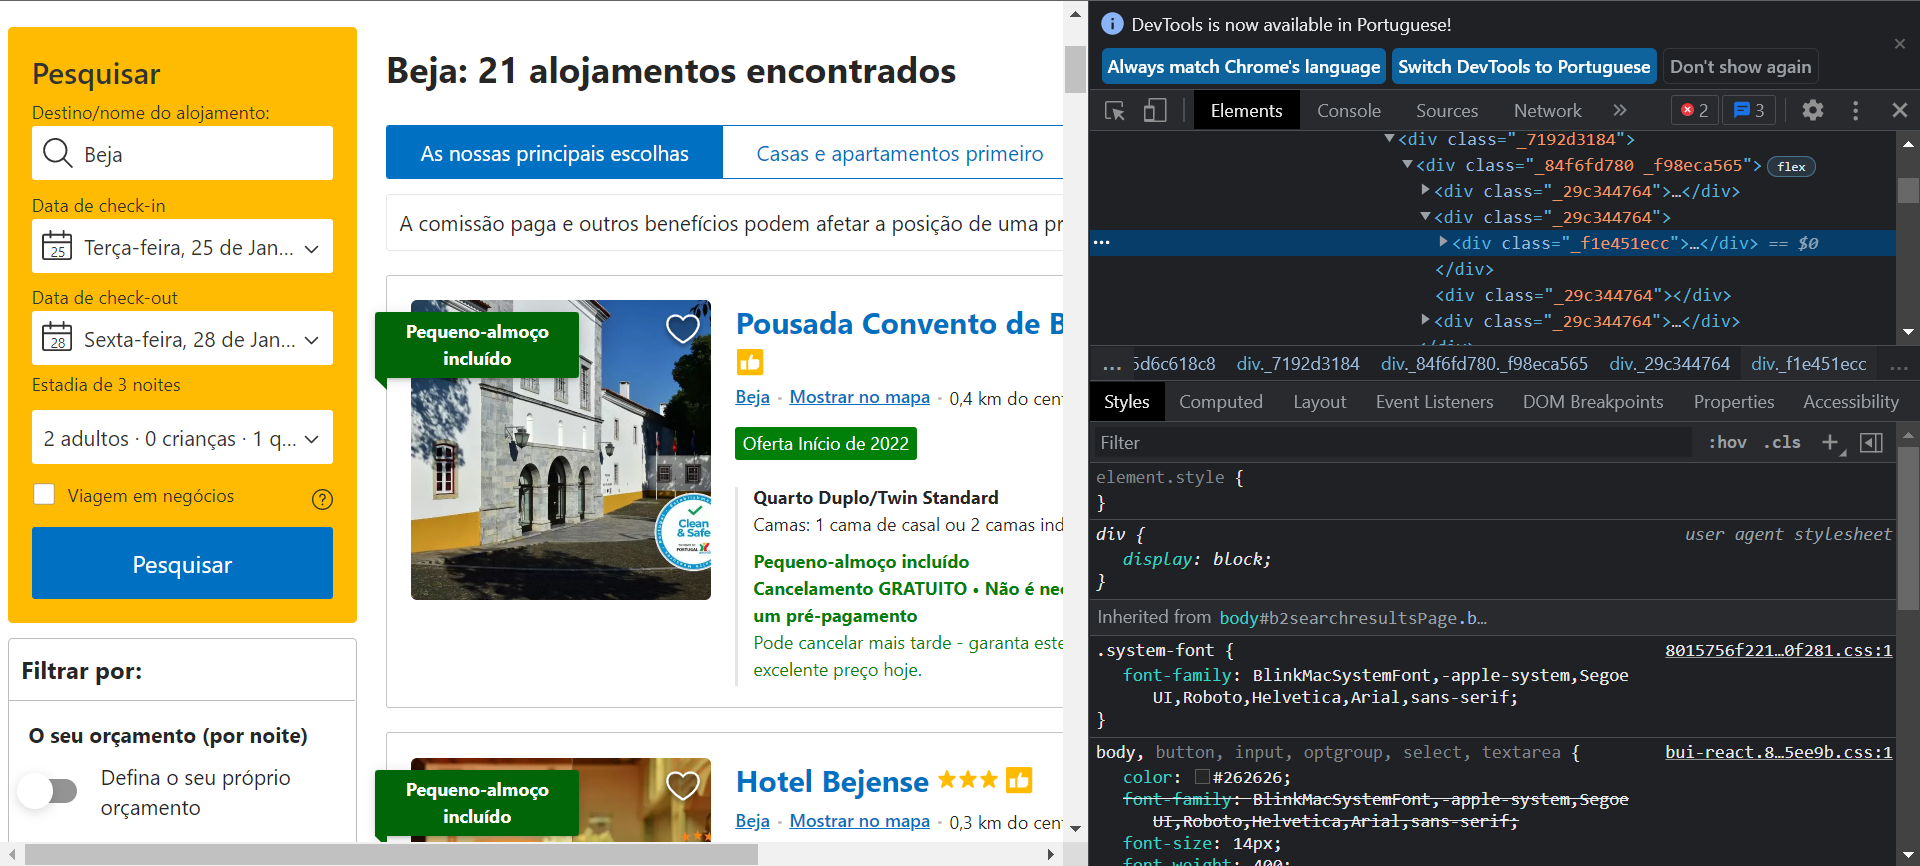
\includegraphics[width=15cm]{1.PNG}
    \caption{Site Booking.com ao usar a ferramenta inspecionar}
    \label{fig:my_label}
\end{figure}

\begin{figure}[!htb]
No código foi implementado as bibliotecas BeautifulSoup para facilitar a tarefa de realizar o "web-scraping".
    \centering
    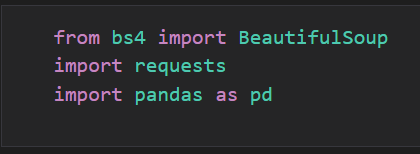
\includegraphics[width=15cm]{2.PNG}
    \caption{"Import" de algumas das bibliotecas necessárias}
    \label{fig:my_label}
\end{figure}

\begin{figure}[!htb]
A partir do "website" ao inspecionar a página era possível retirar os headers que eram valores necessários na realização do "web-scrapping". Também é realizado o pedido HTTP e juntou-se a informação com a biblioteca "BeautifulSoup".
    \centering
    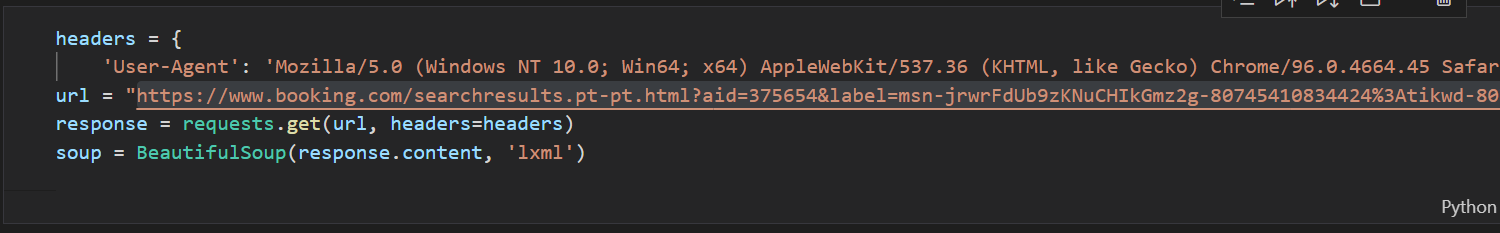
\includegraphics[width=15cm]{3.PNG}
    \caption{"Import" de algumas das bibliotecas necessárias}
    \label{fig:my_label}
\end{figure}

\newpage

\begin{figure}[!htb]
Foram criados diferentes arrays para receber as informações e posteriormente colocada a respetiva informação em cada um deles.
    \centering
    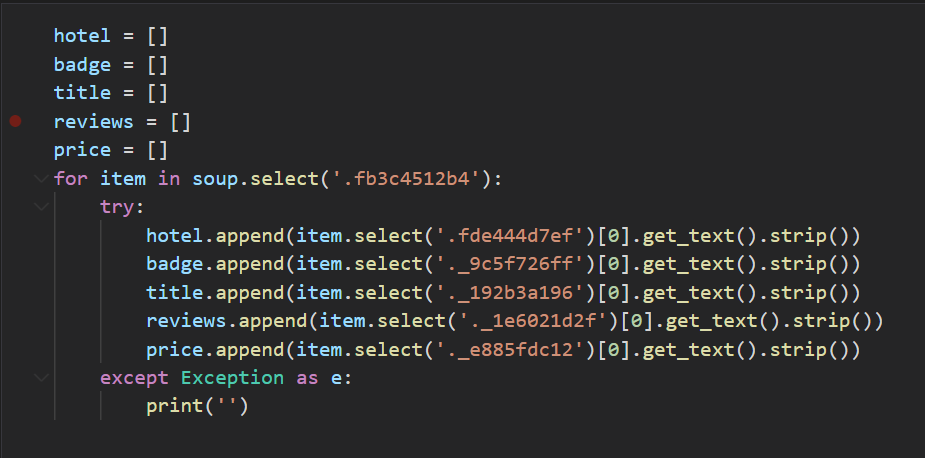
\includegraphics[width=15cm]{4.PNG}
    \caption{"Import" de algumas das bibliotecas necessárias}
    \label{fig:my_label}
\end{figure}

\begin{figure}[!htb]
Devido a alguns "arrays" conterem mais informação, possivelmente devido a algum tipo de informação adicional que possa estar em algum hótel especificamente, para preveneir erros, foi feito um pequeno código para que todos os "arrays" contenham as mesmas dimensões.
    \centering
    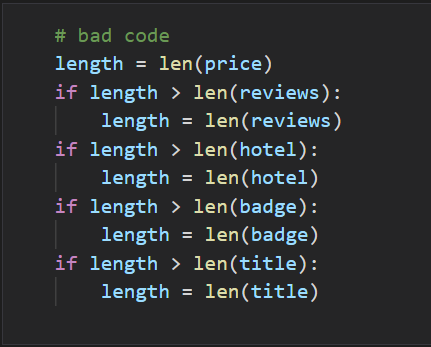
\includegraphics[width=15cm]{5.PNG}
    \caption{"Import" de algumas das bibliotecas necessárias}
    \label{fig:my_label}
\end{figure}

\newpage

\begin{figure}[!htb]
Por fim todos os resultados contidos nos "arrays" foram guardados num ficheiro .csv denominado "listtable.csv".
    \centering
    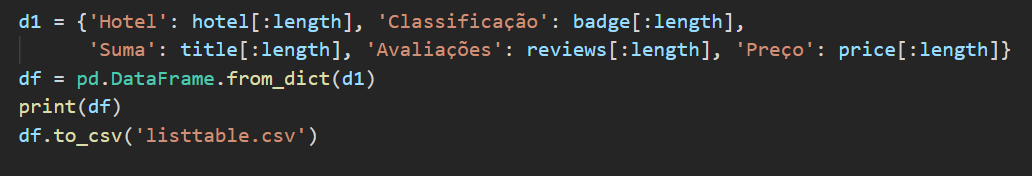
\includegraphics[width=15cm]{6.PNG}
    \caption{"Import" de algumas das bibliotecas necessárias}
    \label{fig:my_label}
\end{figure}

\begin{figure}[!htb]
Alguns dos resultados dos hóteis em Beja.
    \centering
    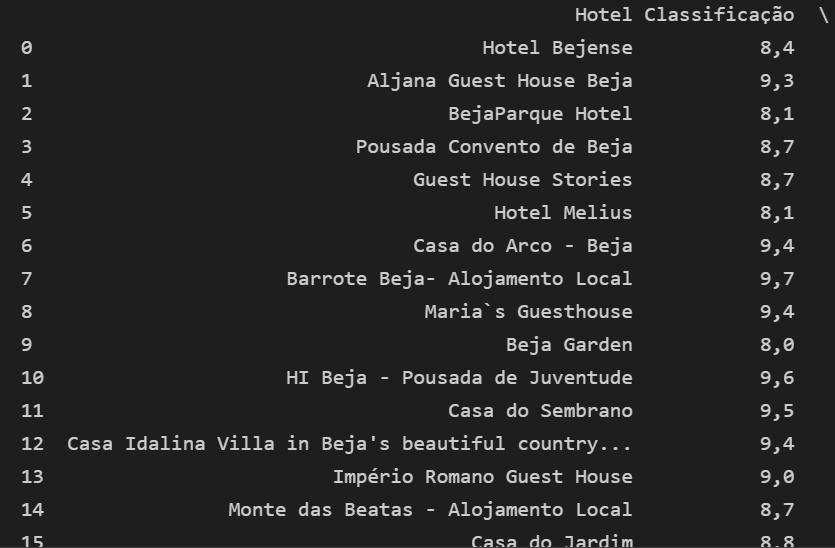
\includegraphics[width=15cm]{7.PNG}
    \caption{"Import" de algumas das bibliotecas necessárias}
    \label{fig:my_label}
\end{figure}

\newpage

\begin{figure}[!htb]
Construção dos links para realizar o "web-scraping" das "reviews" de cada hotel.
    \centering
    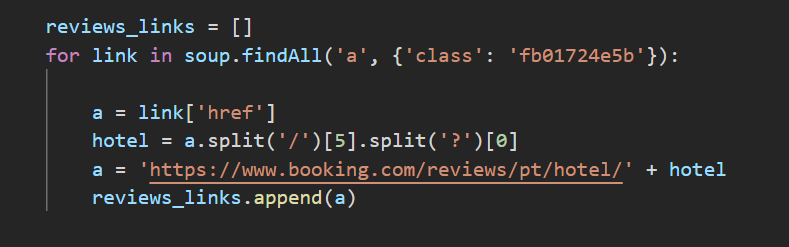
\includegraphics[width=15cm]{8.PNG}
    \caption{"Import" de algumas das bibliotecas necessárias}
    \label{fig:my_label}
\end{figure}

\newpage

\begin{figure}[!htb]
Foi realizado o pedido "HTTP" e juntado á biblioteca "BeautifulSoup" para aceder ás "reviews" de cada site e todos os valores foram salvos no formato .csv.
    \centering
    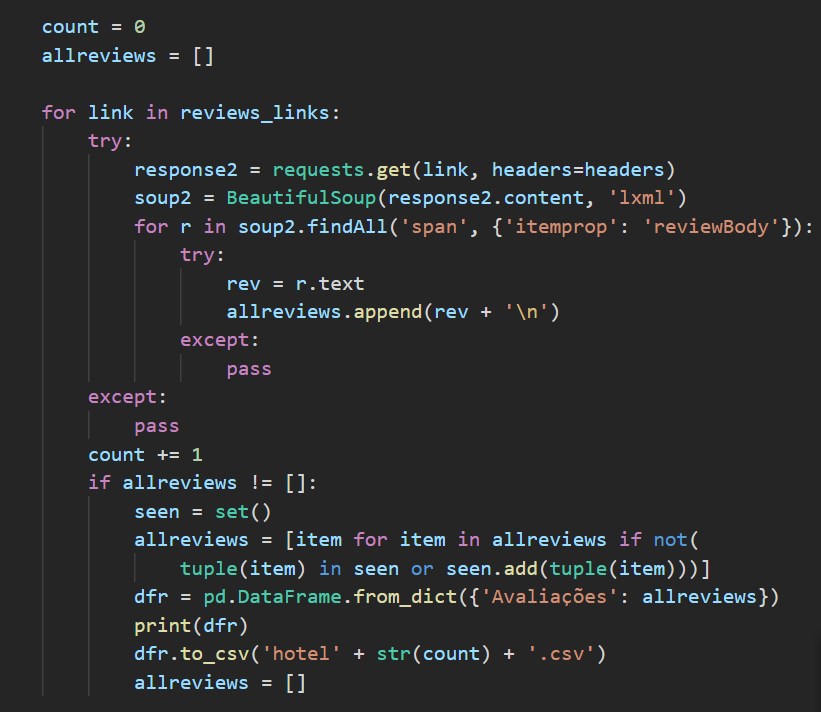
\includegraphics[width=15cm]{9.PNG}
    \caption{"Import" de algumas das bibliotecas necessárias}
    \label{fig:my_label}
\end{figure}

\newpage

\begin{figure}[!htb]
Algumas das "reviews" de um dos sites disponíveis.
    \centering
    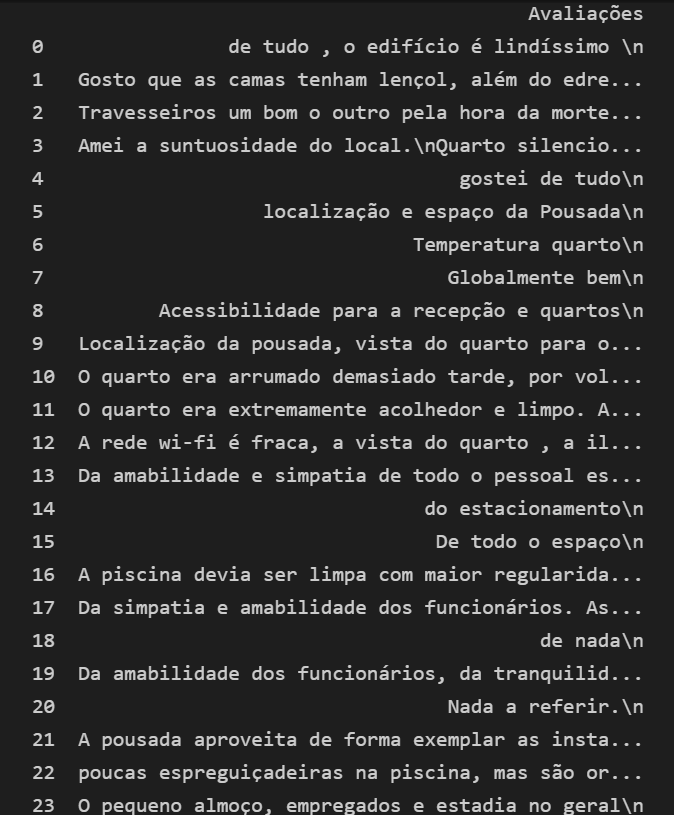
\includegraphics[width=15cm]{10.PNG}
    \caption{"Import" de algumas das bibliotecas necessárias}
    \label{fig:my_label}
\end{figure}

\newpage

\subsubsection{Hotéis}

\begin{table}[!ht]
  \centering
  \begin{tabular}{|l|l|l|l|}
  \hline
      ~ & Hotel & Classificação & Preço \\ \hline
      0 & Hotel Bejense & "8,4" & 189 \\ \hline
      1 & Aljana Guest House Beja & "9,3" & 330 \\ \hline
      2 & BejaParque Hotel & "8,1" & 255 \\ \hline
      3 & Pousada Convento de Beja & "8,7" & 270 \\ \hline
      4 & Guest House Stories & "8,7" & 135 \\ \hline
      5 & Hotel Melius & "8,1" & 242 \\ \hline
      6 & Casa do Arco - Beja & "9,4" & 210 \\ \hline
      7 & Barrote Beja- Alojamento Local & "9,7" & 255 \\ \hline
      8 & Maria`s Guesthouse & "9,4" & 226 \\ \hline
      9 & Beja Garden & "8,0" & 90 \\ \hline
      10 & HI Beja - Pousada de Juventude & "9,6" & 327 \\ \hline
      11 & Casa do Sembrano & "9,5" & 330 \\ \hline
      12 & Casa Idalina Villa in Beja's beautiful countryside & "9,4" & 210 \\ \hline
      13 & Império Romano Guest House & "9,0" & 150 \\ \hline
      14 & Monte das Beatas - Alojamento Local & "8,7" & 306 \\ \hline
      15 & Casa do Jardim & "8,8" & 270 \\ \hline
      16 & Casa das Histórias & "8,9" & 195 \\ \hline
      17 & Casa Centro Histórico Beja - Castelo & "7,9" & 180 \\ \hline
      18 & Quinta do Castelo & "9,0" & 214 \\ \hline
      19 & Casa do Avô Zé & "8,1" & 174 \\ \hline
      20 & Suite na Praça da República & "8,7" & 228 \\ \hline
      21 & Herdade da Diabroria - Agroturismo & "8,8" & 285 \\ \hline
      22 & Herdade do Vau & "7,8" & 270 \\ \hline
      23 & Monte da Corte Ligeira & "8,3" & 150 \\ \hline
  \end{tabular}
        \caption{Tabela com todos os hotéis de Beja retirados do Booking.com}
\end{table}

\newpage

\subsection{Resultados}

\begin{table}[!ht]
  \centering
  \begin{tabular}{|p{50}|p{352}|}
  \hline
      Nº Opinião & Opiniões \\ \hline
      0 & A localização é excelente assim como as condições do espaço. Local muito bem cuidado e apelativo. Fomos muito bem recebidos. A casa estava muito bem equipada. Muito obrigada, Catarina. \\ \hline
      1 & Nada digno de registo. \\ \hline
      2 & A simpatia da Sra Catarina foi fantástica. A casa e as acomodações corresponderam ás expetivas e relação qualidade preço foi perfeita. A localização é óptima, apesar de algum barulho das viaturas que passam junto ás janelas dos quartos. Beja é uma cidade fantástica e voltaremos concerteza. Recomendo. \\ \hline
      3 & Localização excelente, apartamento espaçoso, e totalmente equipado.
      O facto de ser uma construção antiga, cria um ambiente muito peculiar, além de que a expessura das paredes ajuda na questão da temperatura (estivémos no verão, portanto a casa não era quente apesar dos 30 e tal graus na rua).
      \\ \hline
      4 & A localização é impecável mesmo no centro histórico de Beja. Casa Limpa e organizada. Dona super prestável e e simpática. \\ \hline
      5 & De noite ouve-se o barulho da rua com muita facilidade. \\ \hline
      6 & A casa está muito perto do castelo e está muito bem decorada e limpa. Muito agradável!  \\ \hline
      7 & O dono não tem culpa mas a zona não é muito bem frequentada á noite \\ \hline
      8 & A casa é muito gira e funcional! \\ \hline
      9 & Casa muito agradável e bem situada.  Os anfitriães são simpáticos e disponíveis. Cozinha muito bem equipada e casa de banho excelente. \\ \hline
      10 & Da localização, da relação preço/qualidade que entendo adequada.  \\ \hline
      11 & Localização no centro histórico tem vantagens (centralidade) e desvantagens (dificuldades de estacionamento). \\ \hline
      12 & Localização, decoração, conforto, organização do espaço e o gosto cuidado na decoração. \\ \hline
      13 & Não tinha microondas. \\ \hline
      14 & Localização, estacionamento perto, a decoração do alojamento, ter máquina de lavar roupa deu muito geito. \\ \hline
      15 & Virado para duas ruas públicas isso condiciona a entrada de luz e de ventilação em casa pela noção de segurança; 
      Existem algumas infiltrações junto ao pavimento nalgumas divisões, fruto da data de construção e ser uma casa térrea;
      Haver imenso equipamento de cozinha, de limpeza, de menage, mas não haver uma pastilha para a máquina de lavar roupa (mero detalhe).
      \\ \hline
      16 & A casa em si é antiga e possui algumas divisões de formatos, alturas, níveis de pavimento e arcadas distintas, o que lhe dão um ar muito original;
      Está bem conservada/renovada, com uma cozinha bastante equipada (incluindo lavagem e limpeza), onde é possível de confeccionar, conservar e lavar. 
      A localização na zona histórica de Beja, no meio do casario.
      \\ \hline
      17 & Poderia ter um microondas. \\ \hline
      18 & Muito bem localizado, anfitriões muito simpáticos.
      Muito interessante a manutenção de casa típica alentejana.
      Gostamos todos muito
      \\ \hline
      19 & Gostei de tudo. Não tenho do q reclamar. \\ \hline
      20 & O apartamento é uma graça. Super completo, amplo, decorado com muito bom gosto e jovial! Adorei!!!!! \\ \hline
      21 & Serviço conforto e localização. \\ \hline
      22 & A limpeza poderia ser mais cuidada. Não dar para ligar a chaleira eléctrica porque o quadro não aguentava. O fogão estar rachado não ofereceu muita confiança para cozinhar. \\ \hline
      23 & Da receção, da decoração, da temperatura da casa, o ser uma casa acolhedora situada no coração do centro histórico. \\ \hline
      ... & ...\\ \hline
      28 & De tudo. Um lugar ótimo para uma família passar uns dias, a casa está bem situada e as pessoas muito simpáticas. Um lugar a repetir.  \\ \hline
      
    \end{tabular}
        \caption{Tabela de resultados de algumas "Reviews" para um dos hotéis (hotel18.csv)}
\end{table}

\section{Zomato}

\subsection{Estratégia}

\subsection{Desenvolvimento}

\newpage

\subsubsection{Restaurantes}

\begin{table}[!ht]
  \centering
  \begin{tabular}{|l|l|l|l|}
  \hline
      ~ & Restaurante & Tipo & Preço \\ \hline
      0 & Adega Típica 25 de Abril & "Alentejana, Portuguesa" & 25 \\ \hline
      1 & Dom Dinis & "Bifes, Portuguesa" & 30 \\ \hline
      2 & Sushi Alentejano & "Sushi, Japonesa" & 35 \\ \hline
      3 & Herdade dos Grous & "Contemporânea, Portuguesa" & 60 \\ \hline
      4 & Pulo do Lobo & Portuguesa & 25 \\ \hline
      5 & Bar Parque da Vila Beringel & "Snacks, Bebidas" & 12 \\ \hline
      6 & Figa's & "Pizza, Italiana" & 25 \\ \hline
      7 & Cervejaria Portugalo & "Portuguesa, Bebidas, Petiscos" & 25 \\ \hline
      8 & Entre Arcos & "Portuguesa, Grelhados" & 25 \\ \hline
      9 & Aperitivo & "Bebidas, Portuguesa" & 20 \\ \hline
      10 & O Arbitro & Portuguesa & 25 \\ \hline
      11 & Café Central & "Snacks, Bebidas, Portuguesa" & 15 \\ \hline
      12 & Gatus Cervejaria Alentejana & "Alentejana, Portuguesa, Marisqueira" & 25 \\ \hline
      13 & Hamburgueria da Avenida & Hamburgueria & 25 \\ \hline
      14 & Casa de Pasto O Forno & "Snacks, Bebidas, Portuguesa" & 12 \\ \hline
      15 & Tennis Courts Club & Portuguesa & 25 \\ \hline
      16 & Cervejaria Mira Serra & "Marisqueira, Portuguesa" & 40 \\ \hline
      17 & Espelho d'Água & Portuguesa & 25 \\ \hline
      18 & TEM Avondo & "Portuguesa, Alentejana" & 25 \\ \hline
      19 & Menau & Portuguesa & 25 \\ \hline
      20 & Toy Faróis & "Portuguesa, Grelhados" & 25 \\ \hline
      21 & Taberna A Pipa & "Alentejana, Portuguesa, Petiscos" & 25 \\ \hline
      22 & Pizzeria Milano & "Pizza, Italiana, Portuguesa" & 25 \\ \hline
      23 & Dona Maria Deck & "Portuguesa, Petiscos, Snacks" & 25 \\ \hline
      24 & O Alemão & "Portuguesa, Petiscos, Alentejana" & 25 \\ \hline
      25 & Deliciosa Alvorada & "Portuguesa, Alentejana" & 25 \\ \hline
      26 & Moments IPDJ & Portuguesa & 20 \\ \hline
      27 & Bar Regional & "Bebidas, Snacks" & 6 \\ \hline
      28 & Sushizzaria & "Sushi, Hamburgueria, Pizza" & 30 \\ \hline
      \ldots & \ldots & \ldots & \ldots \\ \hline
      155 & Vegetariano & Vegetariana & 25 \\ \hline
  \end{tabular}
\end{table}

\newpage

\subsection{Resultados}

\newpage

\section{Próximos Passos}

Na seguinte fase de trabalho o grupo irá ter que começar a desenvolver os processos ETL (extract, transform, load) do trabalho já realizado, uma das tarefas será a adaptação de todo o conteúdo textual já armazenado.

\newpage

\section{Conclusão}

Concluindo, este trabalho serviu para aprender o que realmente é o "web-scraping" e todos os usos que ele pode ter para a recolha de dados estruturados da web. Para além de aprender o que ele realmente é, também tivemos a oportunidade de trabalhar com ele e usá-lo num caso prático. Houveram algumas dúvidas principalmente para retirar algumas informações de alguns dos "websites" trabalhados e também na criação do ambiente virtual, porem todas as duvidas foram superadas graças ao trabalho em equipa e pesquisas online, para alem da ajuda da docente responsável pelo projeto. Por fim, achamos que o balanço desta parte do trabalho tenha sido bastante positiva.

\newpage

\section{Webgrafia}

https://www.youtube.com/watch?v=PRkOFgNAkio

Booking.com

\renewcommand{\bibsection}{}
\bibliography{main.bib}

\end{document}
